\chapter{Overview of existing benchmark solutions}

There are number projects that provide input formulas for solvers, in order to test their performance. The majority of them provide pregereneted files grouped in categories, some of them hosts websites with problem (and optionally solutions) database and very few of them generate input formulas on demand. A selection of different benchmark solutions is described in this chapter.

\section{SMT-LIB}
\label{sec:SMTLIBBenchmarks}

As described in section \ref{sec:SMTLIB}, SMT-LIB is both standard for encoding formulas and database of benchmarks. There are 2 main categories of benchmarks: incremental and non-incremental. This enables testing solvers in different scenarios. Next benchmarks are divided into different logics (sublogics) what in the end gives several dozen of different categories. Sublogics are logics that allow only certain theories. For example one sublogic is 
\begin{itemize}
  \item logic with closed linear formulas over linear integer arithmetic (SMT-LIB calls it LIA)
  \item logic with closed linear formulas in linear real arithmetic (LRA) 
  \item logic with quantifier-free integer arithmetic (QF\_NIA) and more
\end{itemize}

\section{SATLIB}

SATLIB \cite{Hol00} is a collection of benchmark problems, solvers, and tools used for SAT related research. Its collection of pregereneted benchmarks is provided in propositional logic (DIMACS format). Benchmarks are grouped into categories, to name a few:
\begin{itemize}
\item uniform random-3-SAT
\item random-3-SAT instances and backbone-minimal sub-instances
\item random-3-SAT instances with controlled backbone size
\item "flat" graph colouring
\item "morphed" graph colouring and more
\end{itemize}

\section{Tough SAT}

Tough SAT \cite{ToughSAT} is an online platform that can generate boolean CNF formulas that encode predefined problems. Problems are represented in propositional logic (DIMACS format). Although Tough SAT is in fact generator it supports only several predefined problems. Mentioned problems are:
\begin{itemize}
  \item factoring -- generate a CNF formula whose satisfying assignment encodes two non-trivial factors of the product $Factor1*Factor2$ (if there exist any). $Factor1$ and $Factor2$ is provided by user.
  \item random subset sum -- generate a random subset sum instance (the ground set is of size Set Size and whose elements are random positive integers less than Max Number, and the target number is the sum of a random subset of the ground set), and encode the instance as a boolean CNF formula
  \item manual subset sum -- variation of above
  \item random -- k-SAT generate a random k-SAT boolean formula with the specified number of variables and clauses
  \item cocktail SAT -- mix of all of above
\end{itemize}

% \item PySAT\footnote{\url{https://pysathq.github.io/}} -- is a toolkit, which aims at providing a simple and unified interface to a number of SAT solvers as well as to a variety pseudo-Boolean encodings. Rather than generating benchmarks this tool is useful when there is a need to access several solvers with unified interface.

\section{CNFgen}

CNFGen \cite{CNFGen} is a python script that produces combinatorial benchmarks in propositional logic (DIMACS format). These benchmarks come mostly from research in proof complexity. CNFGen can generate random formulas but also number of predefined problems:
\begin{itemize}
  \item pigeonhole principle problem -- the formula states that if $n$ items are put into $m$ containers, with $n > m$,  then at least one container must contain more than one item
  \item parity principle problem -- the formula claims that $N$ elements can be matched in pairs
  \item k-clique problem -- the formula claims that there is no clique of size at least $k$ in the input graph $G$. and more
\end{itemize}

\section{Thousands of Problems for Theorem Provers}

As described in section \ref{sec:TPTP}, TPTP is both standard and benchmark database. It contains library of problems encoded in TPTP format. Formulas are classified into different domains (groups): LCL - Logic Calculi, COL - Combinatory Logic and more. These formulas can be queried to filter for example formulas from different domains with same number of atoms. 

Next to TPTP library there is \gls{TSTP} - library of solutions produced by various solvers based on mentioned problem database. \gls{TSTP} additionally contains tools for examining and manipulating the solutions. 

In the end in TPTP there is also \gls{TMTP} - a library of models of axiomatizations for \gls{ATP} systems. Together TPTP, TSTP and TMTP create set of tools for benchmarking, validating and comparing solvers.

\section{The need of new solution}

Although a lot of ready to use benchmarks can be found, there are not a lot of generators. Tough SAT and CNFgen are generators that generate mainly predefined problem with given size, but they operate only in propositional logic. SMT-LIB, SATLIB, TPTP are repositories of benchmarks, not generators itself. Out of mentioned solutions only SMT-LIB and TSTP support first order logic. None of mentioned solutions can generate first order logic formulas. Out of mentioned projects, only CNFGen can produce random formulas.

None of mentioned existing solutions are able to produce random first order logic formulas thus a new solution will be presented in following chapter.



\chapter{Random first order logic formula generator - architecture}
\label{chap:GeneratorArchitecture}

There are 2 parts that together create generator. The main part is $Generator$ (picture \ref{pic:GeneratorOverview}) which is responsible for creating random formula itself and $ExportUtils$ (picture \ref{pic:ExportOverview}) is complementary package responsible encoding formula to \gls{TPTP} format and counting statistics.

The base of $Generator$ is $SyntaxTree$ (described in section \ref{sec:SyntaxTree}) - it defines elements elements of \gls{FOL} in program. Every element defined in $SyntaxTree$ is has at least one corresponding $SubGenerator$ (see section \ref{sec:SubGenerators}), and multiple $SubGenerators$ create $GeneratorPreset$. $GeneratorPreset$ is the element which is going to ensure that generated formula is random within limits. This element is also interface for user (see section \ref{sec:GeneratorPresets}).

\begin{figure}[h]
  \centering
  \begin{subfigure}[b]{0.8\textwidth}
    \centering
    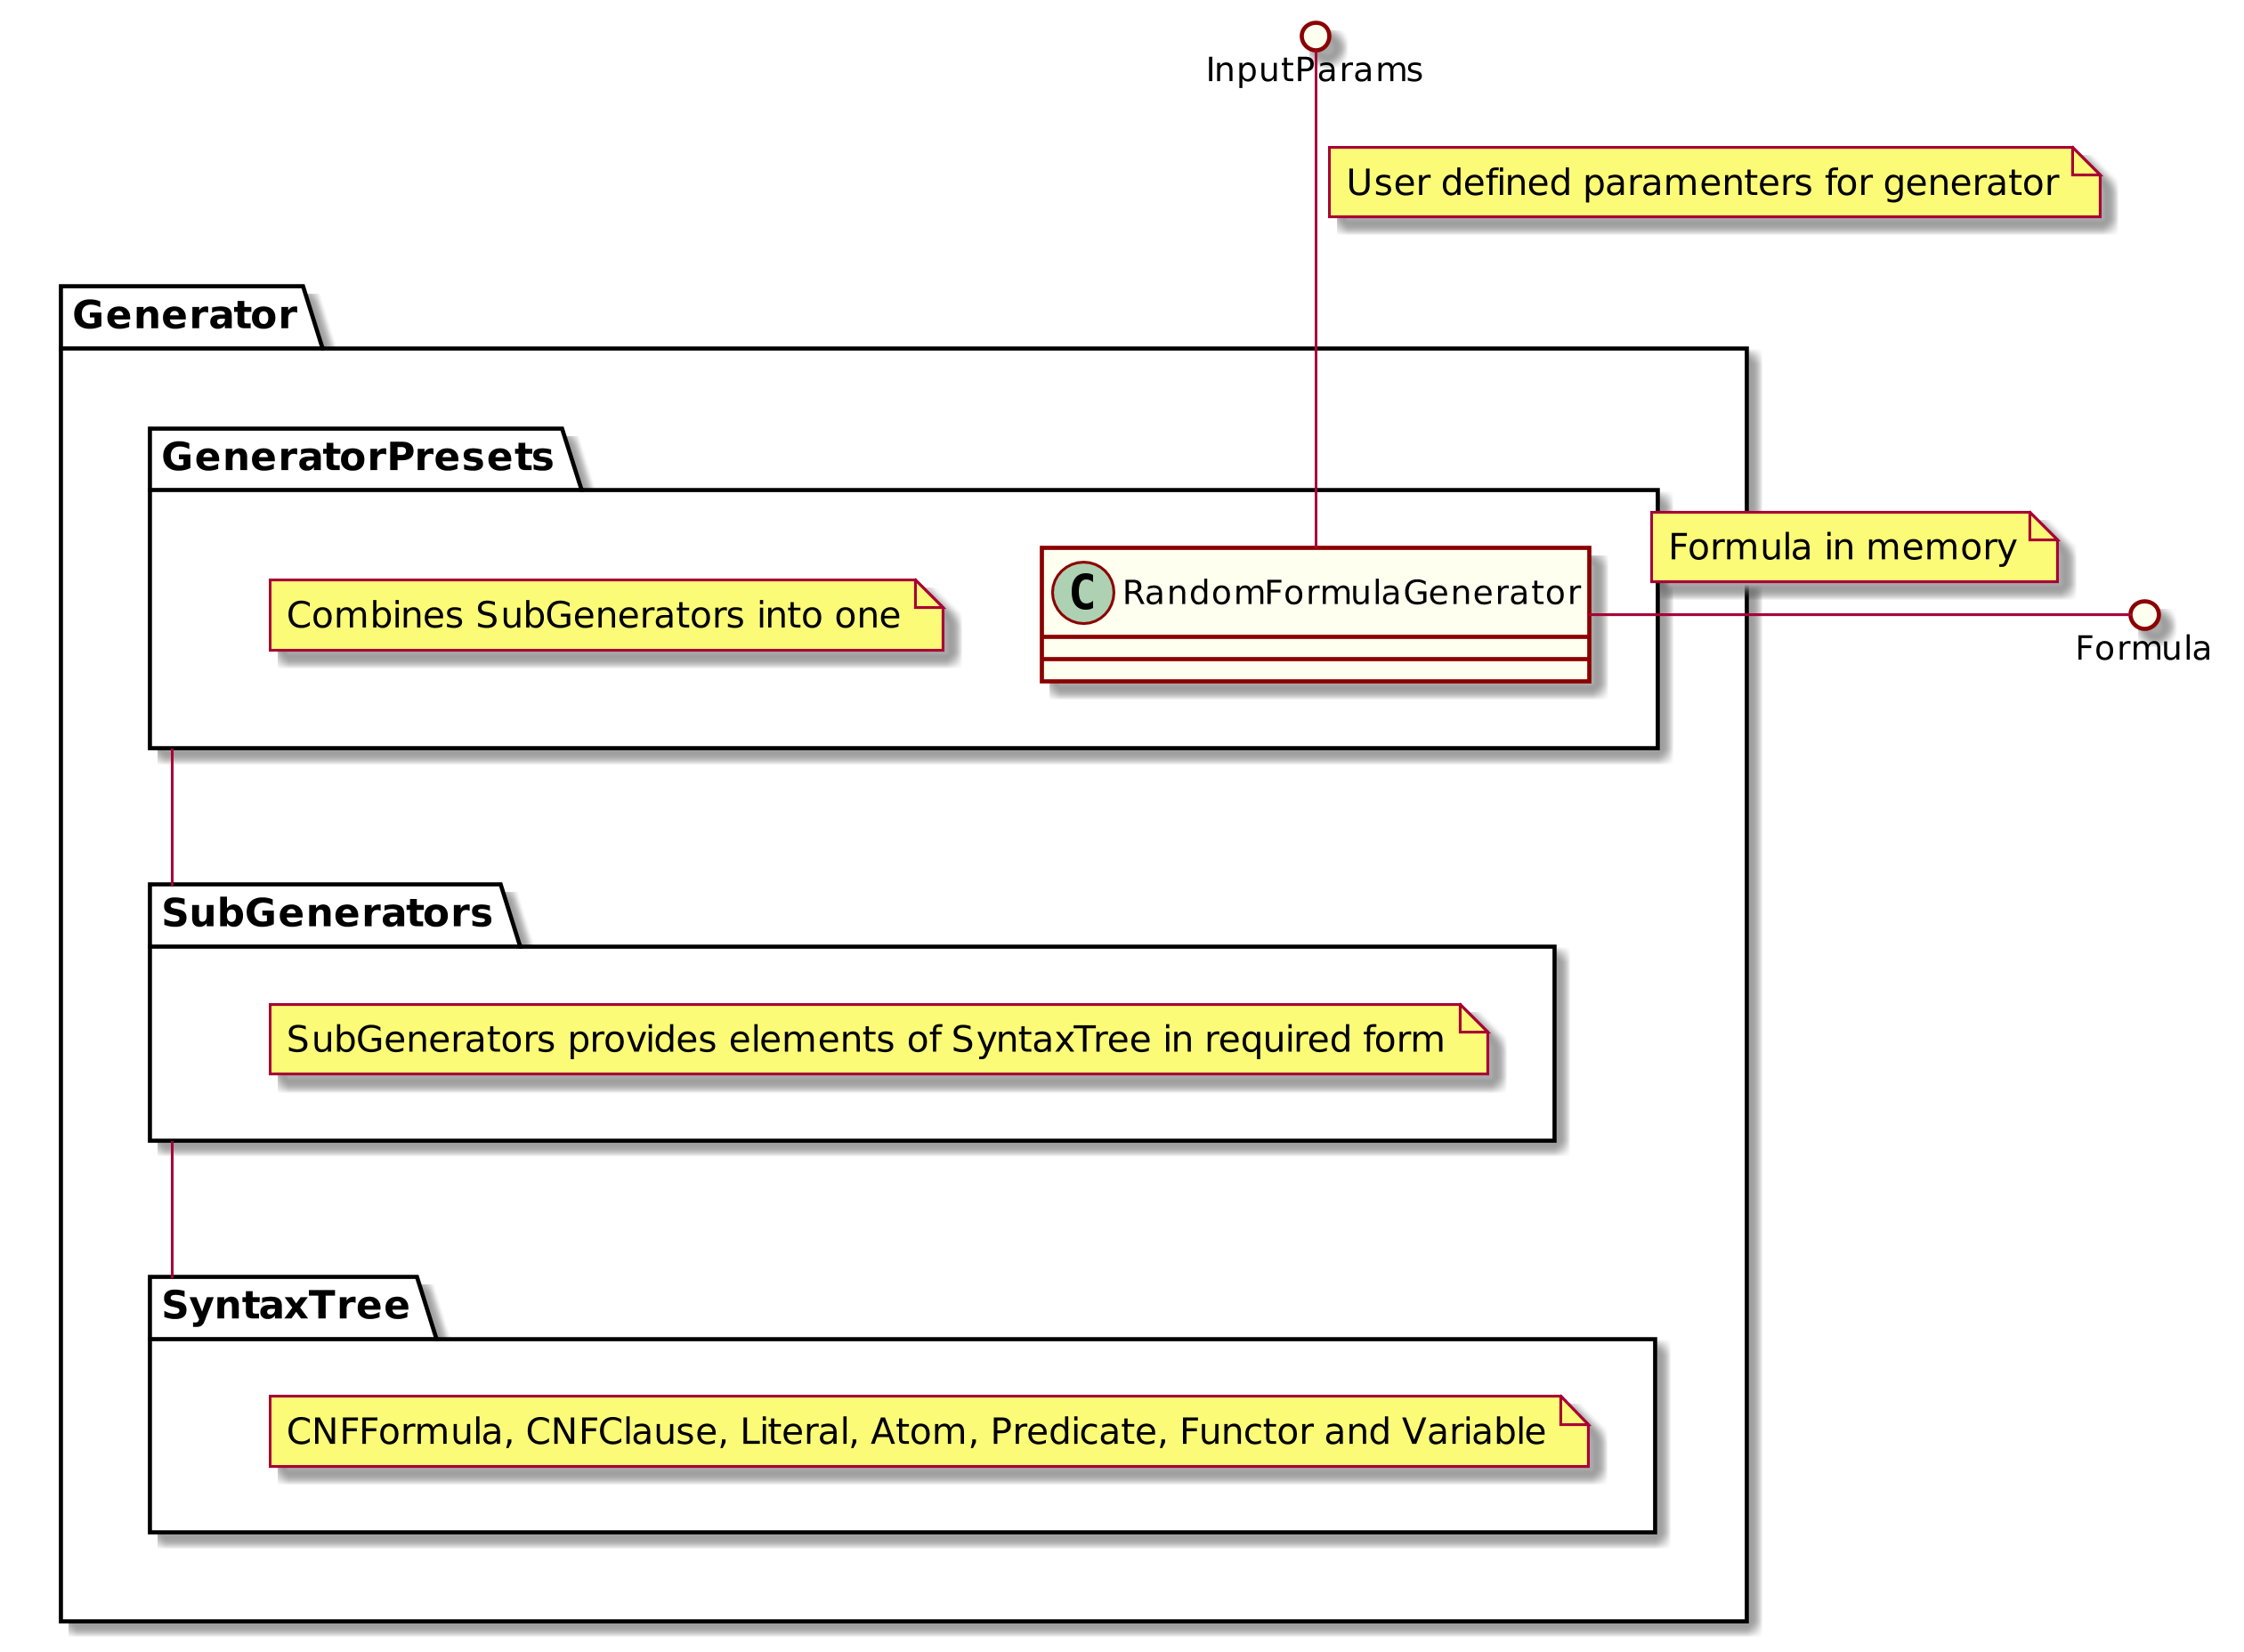
\includegraphics[width=\textwidth]{logic-formula-generator/fol/cnf_generator_overview.png}
    \caption{Overview of formula generation process}
    \label{pic:GeneratorOverview}
  \end{subfigure}

  \begin{subfigure}[b]{0.7\textwidth}
    \centering
    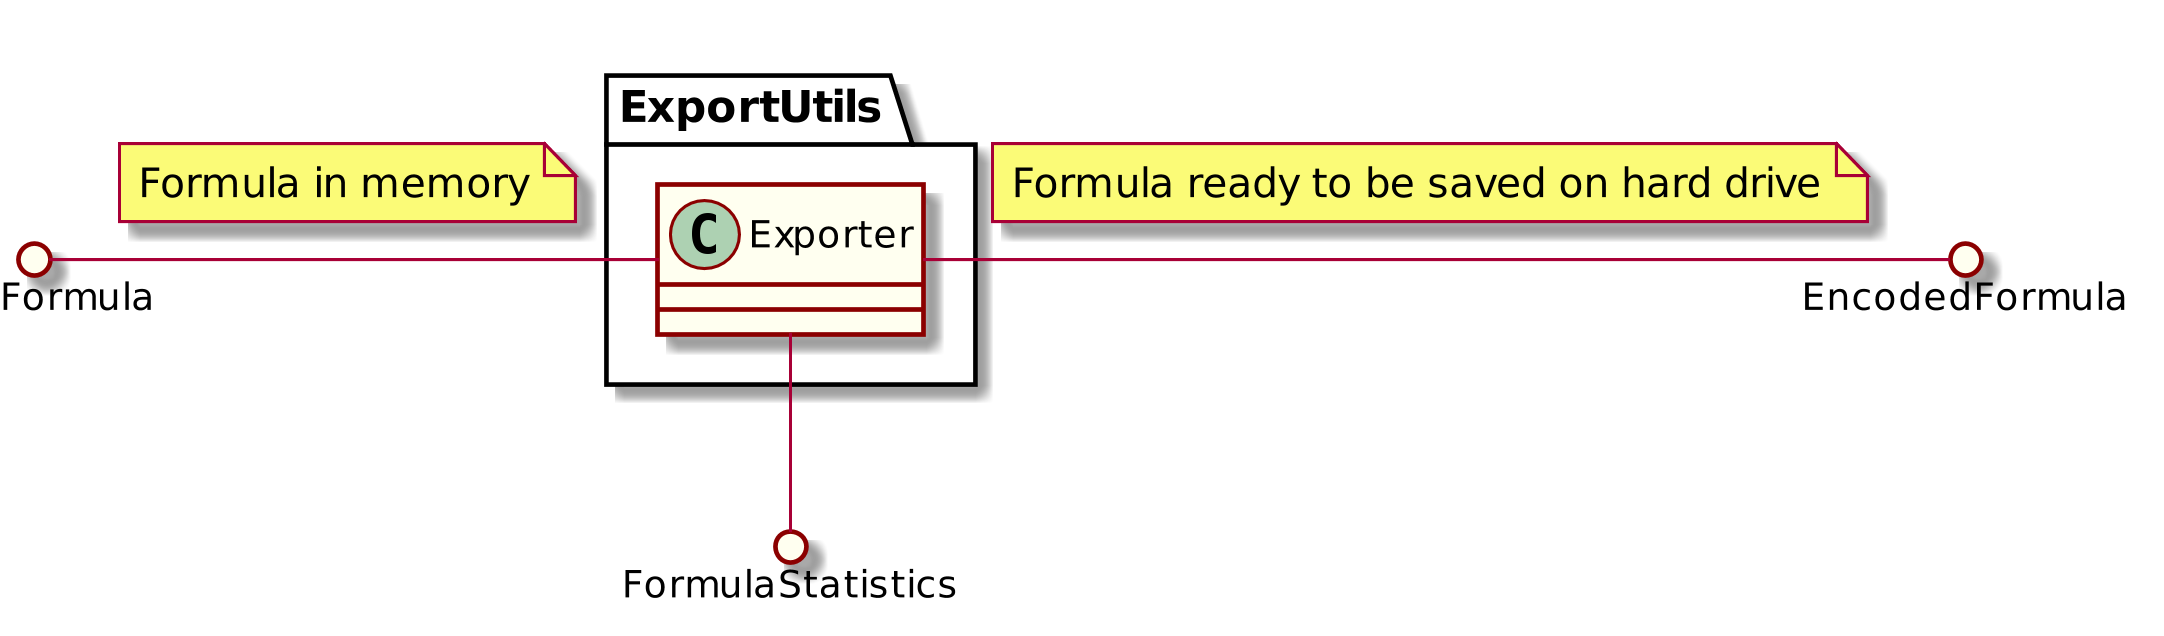
\includegraphics[width=\textwidth]{logic-formula-generator/fol/export_overview.png}
    \caption{Overview of formula exporting process}
    \label{pic:ExportOverview}
  \end{subfigure}
  \caption{Overview of generator architecture}
  \label{pic:ExportAndGeneratorOverview}
\end{figure}

\section{Generator input parameters}
\label{sec:GeneratorParameters}

$Generator$ takes as input user provided parameters and outputs random formula. User provided parameters have 2 flavours. The first set of parameters are not processed in any way, the set "background" for further randomizing formula. These include:
\begin{itemize}
  \item set of variable names $\{'v1','v2',\dots\}$
  \item set of functor names $\{'f1','f2',\dots\}$
  \item set of predicate names $\{'p1','p2',\dots\}$
  \item set of allowed functor arities $a_f = \{0, 1, 2,\dots\}$
  \item maximum recursion depth $n$ for functors
  \item set of allowed predicate arities $a_p = \{0, 1, 2,\dots\}$
  \item set of atom allowed connectives, that is no connective or/and any subset of $AllowedConnectives = \{=, !=, \emptyset\}$
  \item set of allowed clause lengths $ClauseLengths = \{1,2,\dots\}$
  \item amount of literals to be negated
\end{itemize}

Second group of parameters is the main point of interest - these parameters are provided as range of possible values, that user wants to achieve in generated formula:
\begin{itemize}
  \item formula contains from $c_{min}$ to $c_{max}$ clauses
  \item formula contains from $l_{min}$ to $l_{max}$ literals
\end{itemize}

\section{Implementation of syntax tree of first order logic}
\label{sec:SyntaxTree}

Abstract syntax tree of \gls{FOL} is implemented in the same way as mathematical definition, see picture~\ref{pic:fol_elements_class_diagram}. All classes have base class $FolElement$ so that they can be easily identified as element of first order logic and introduce visitor pattern. Visitor pattern is used for exporting formula from intermediate representation to the format of choice (like \gls{TPTP}) as well as counting statistics about generated formula. See for example listing~\ref{lis:TPTPExample} - it is convention from TPTP to store some statistics about file at the beginning of file as comment.

Variable and functor are terms, that is why the inherit from term class. Functor is recursive structure it can contain variable or another term, that is why it is connected with aggregation with term class. Predicate can contain only terms, atom can contain term or predicate, literal can contain only one atom but adds sign to it, clause is one or more literal, CNF formula is one or more clause.

\begin{figure}[h]
\begin{centering}
  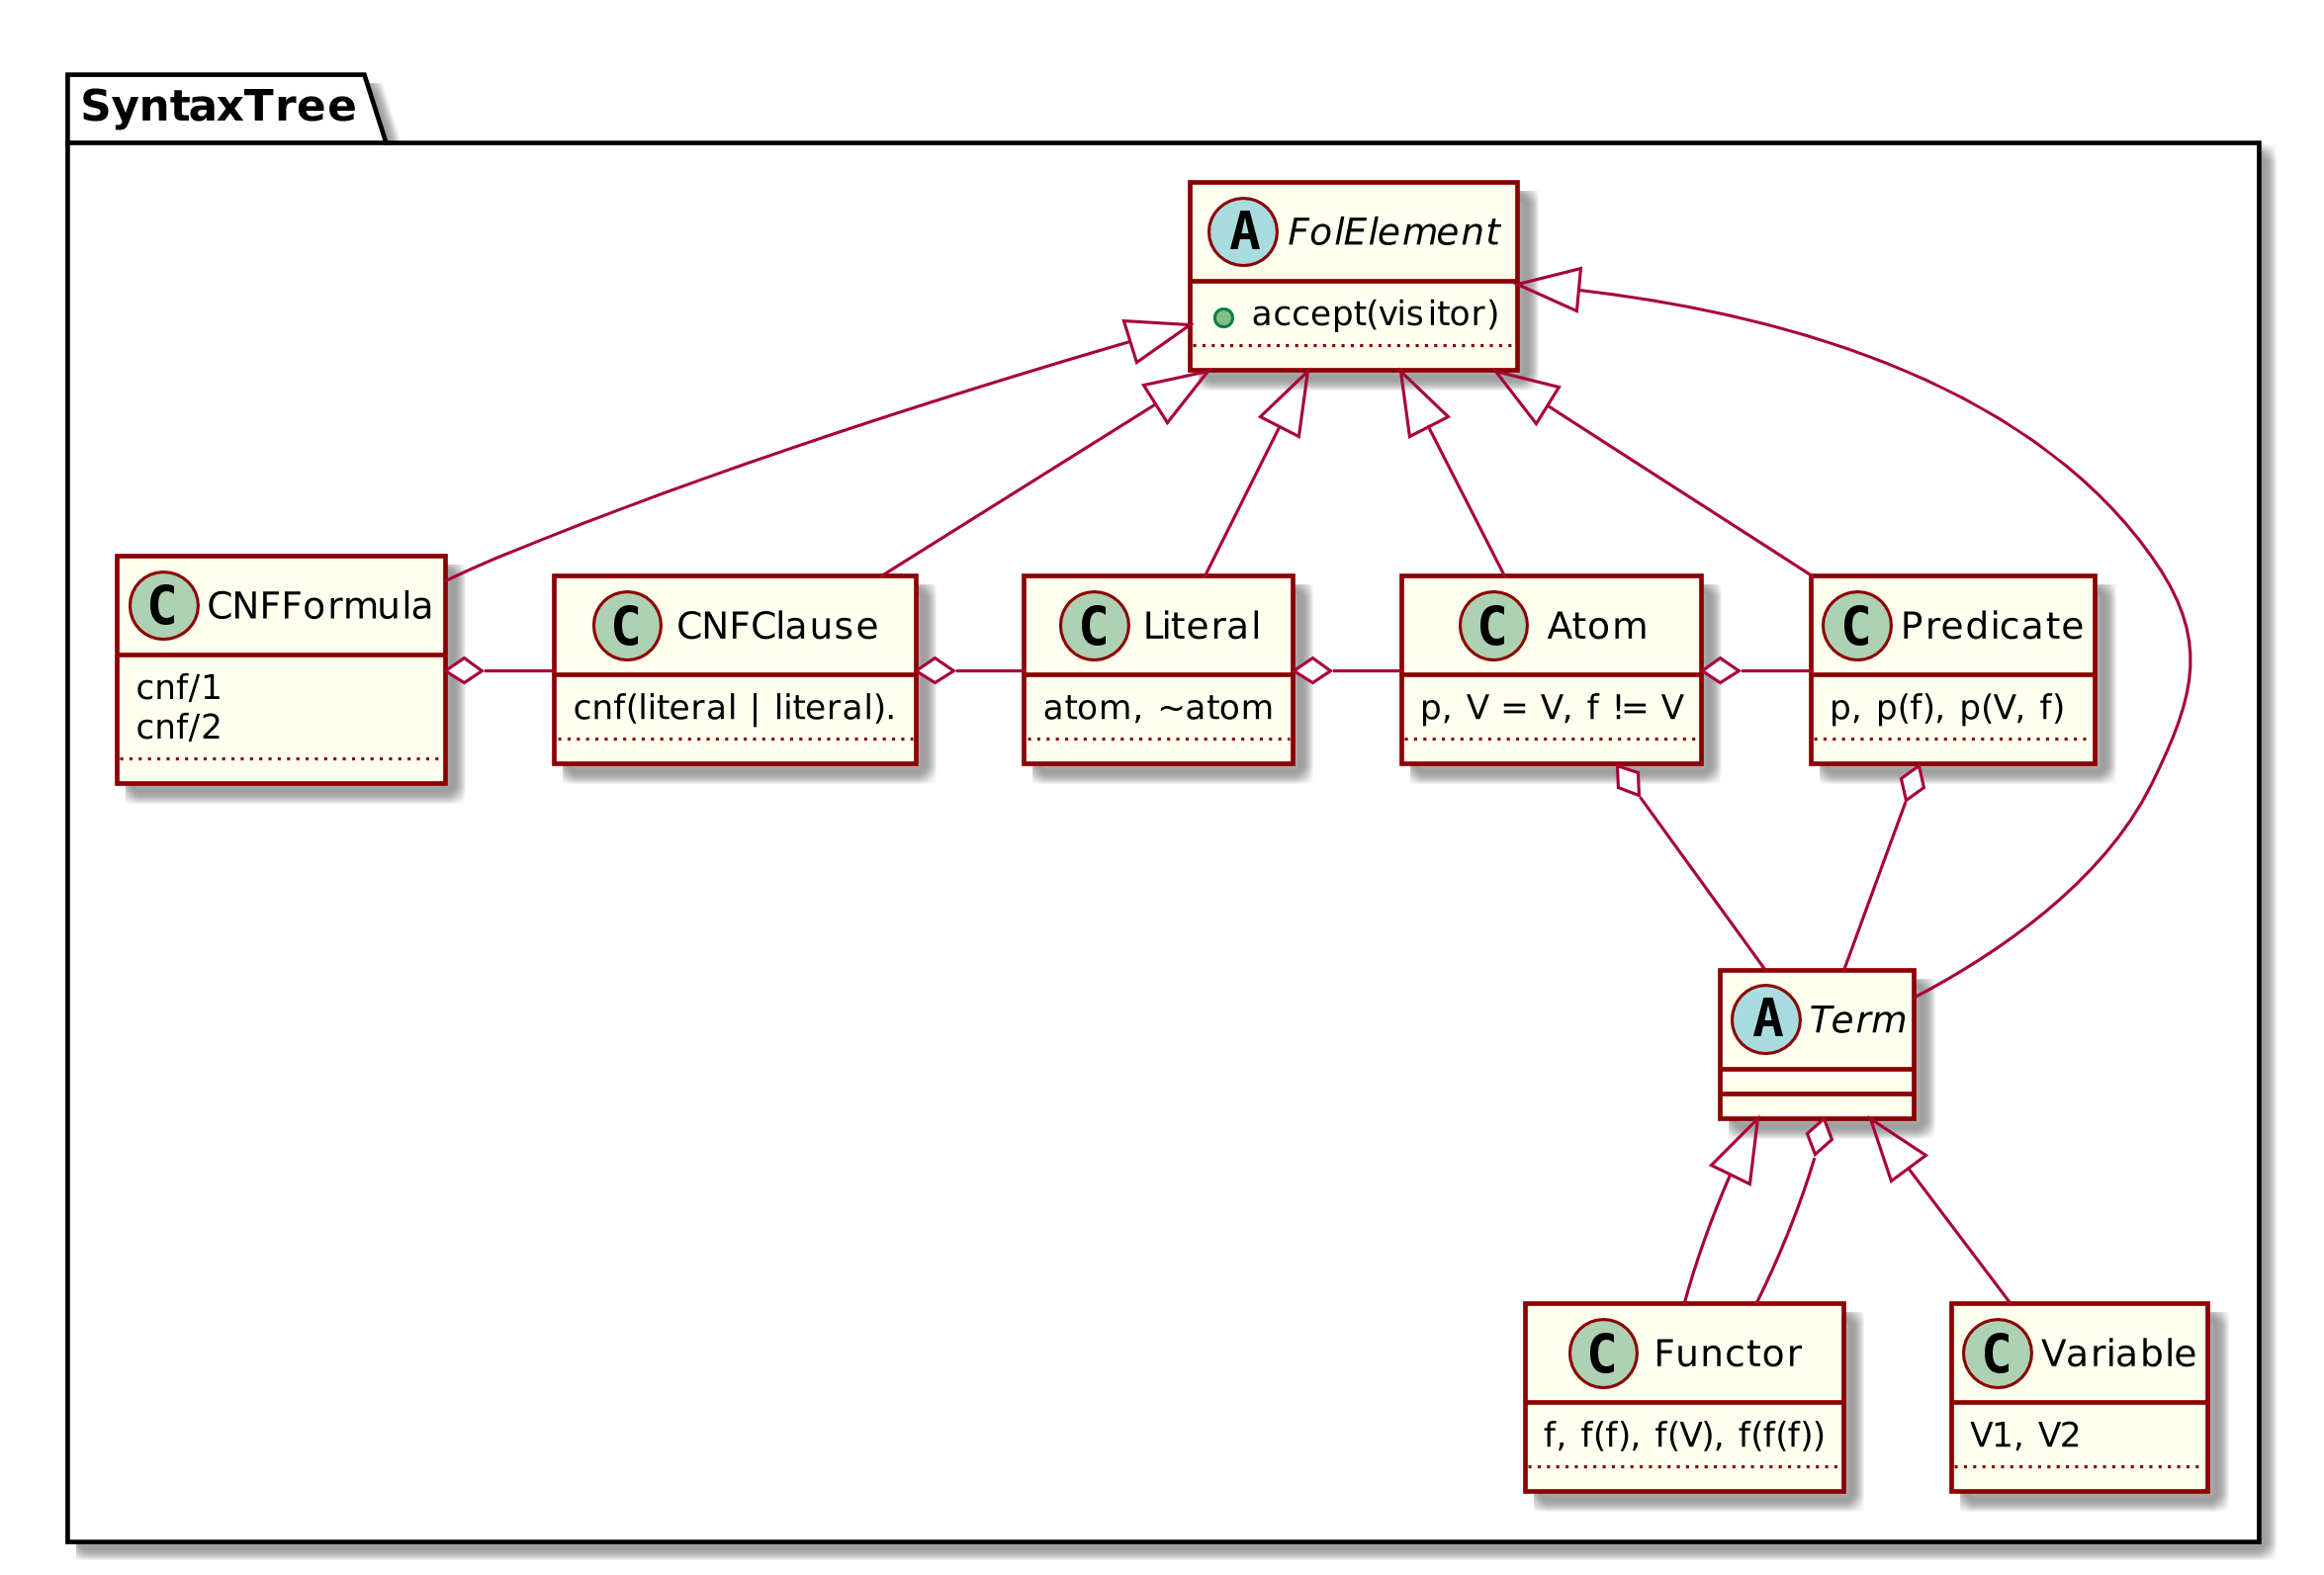
\includegraphics[width=\textwidth]{logic-formula-generator/fol/cnf_fol_elements.png}
  \caption{Class diagram for internal representation of first order logic elements}
  \label{pic:fol_elements_class_diagram}
\end{centering}
\end{figure}

\section{Implementation of SubGenerators}
\label{sec:SubGenerators}

Generators are meant to be used as cascade (picture~\ref{pic:fol_signature_generator_class_diagram}), that is formula generator which provides formulas requires subgenerator which provides clauses, which requires subgenerator which provides literals and so on. This concept ensures that one class has one responsibility. Note that all parameters from described as "background" are passed to subgenerators. Function $generate()$ returns randomized element of syntax tree. 

\begin{figure}[h]
\begin{centering}
  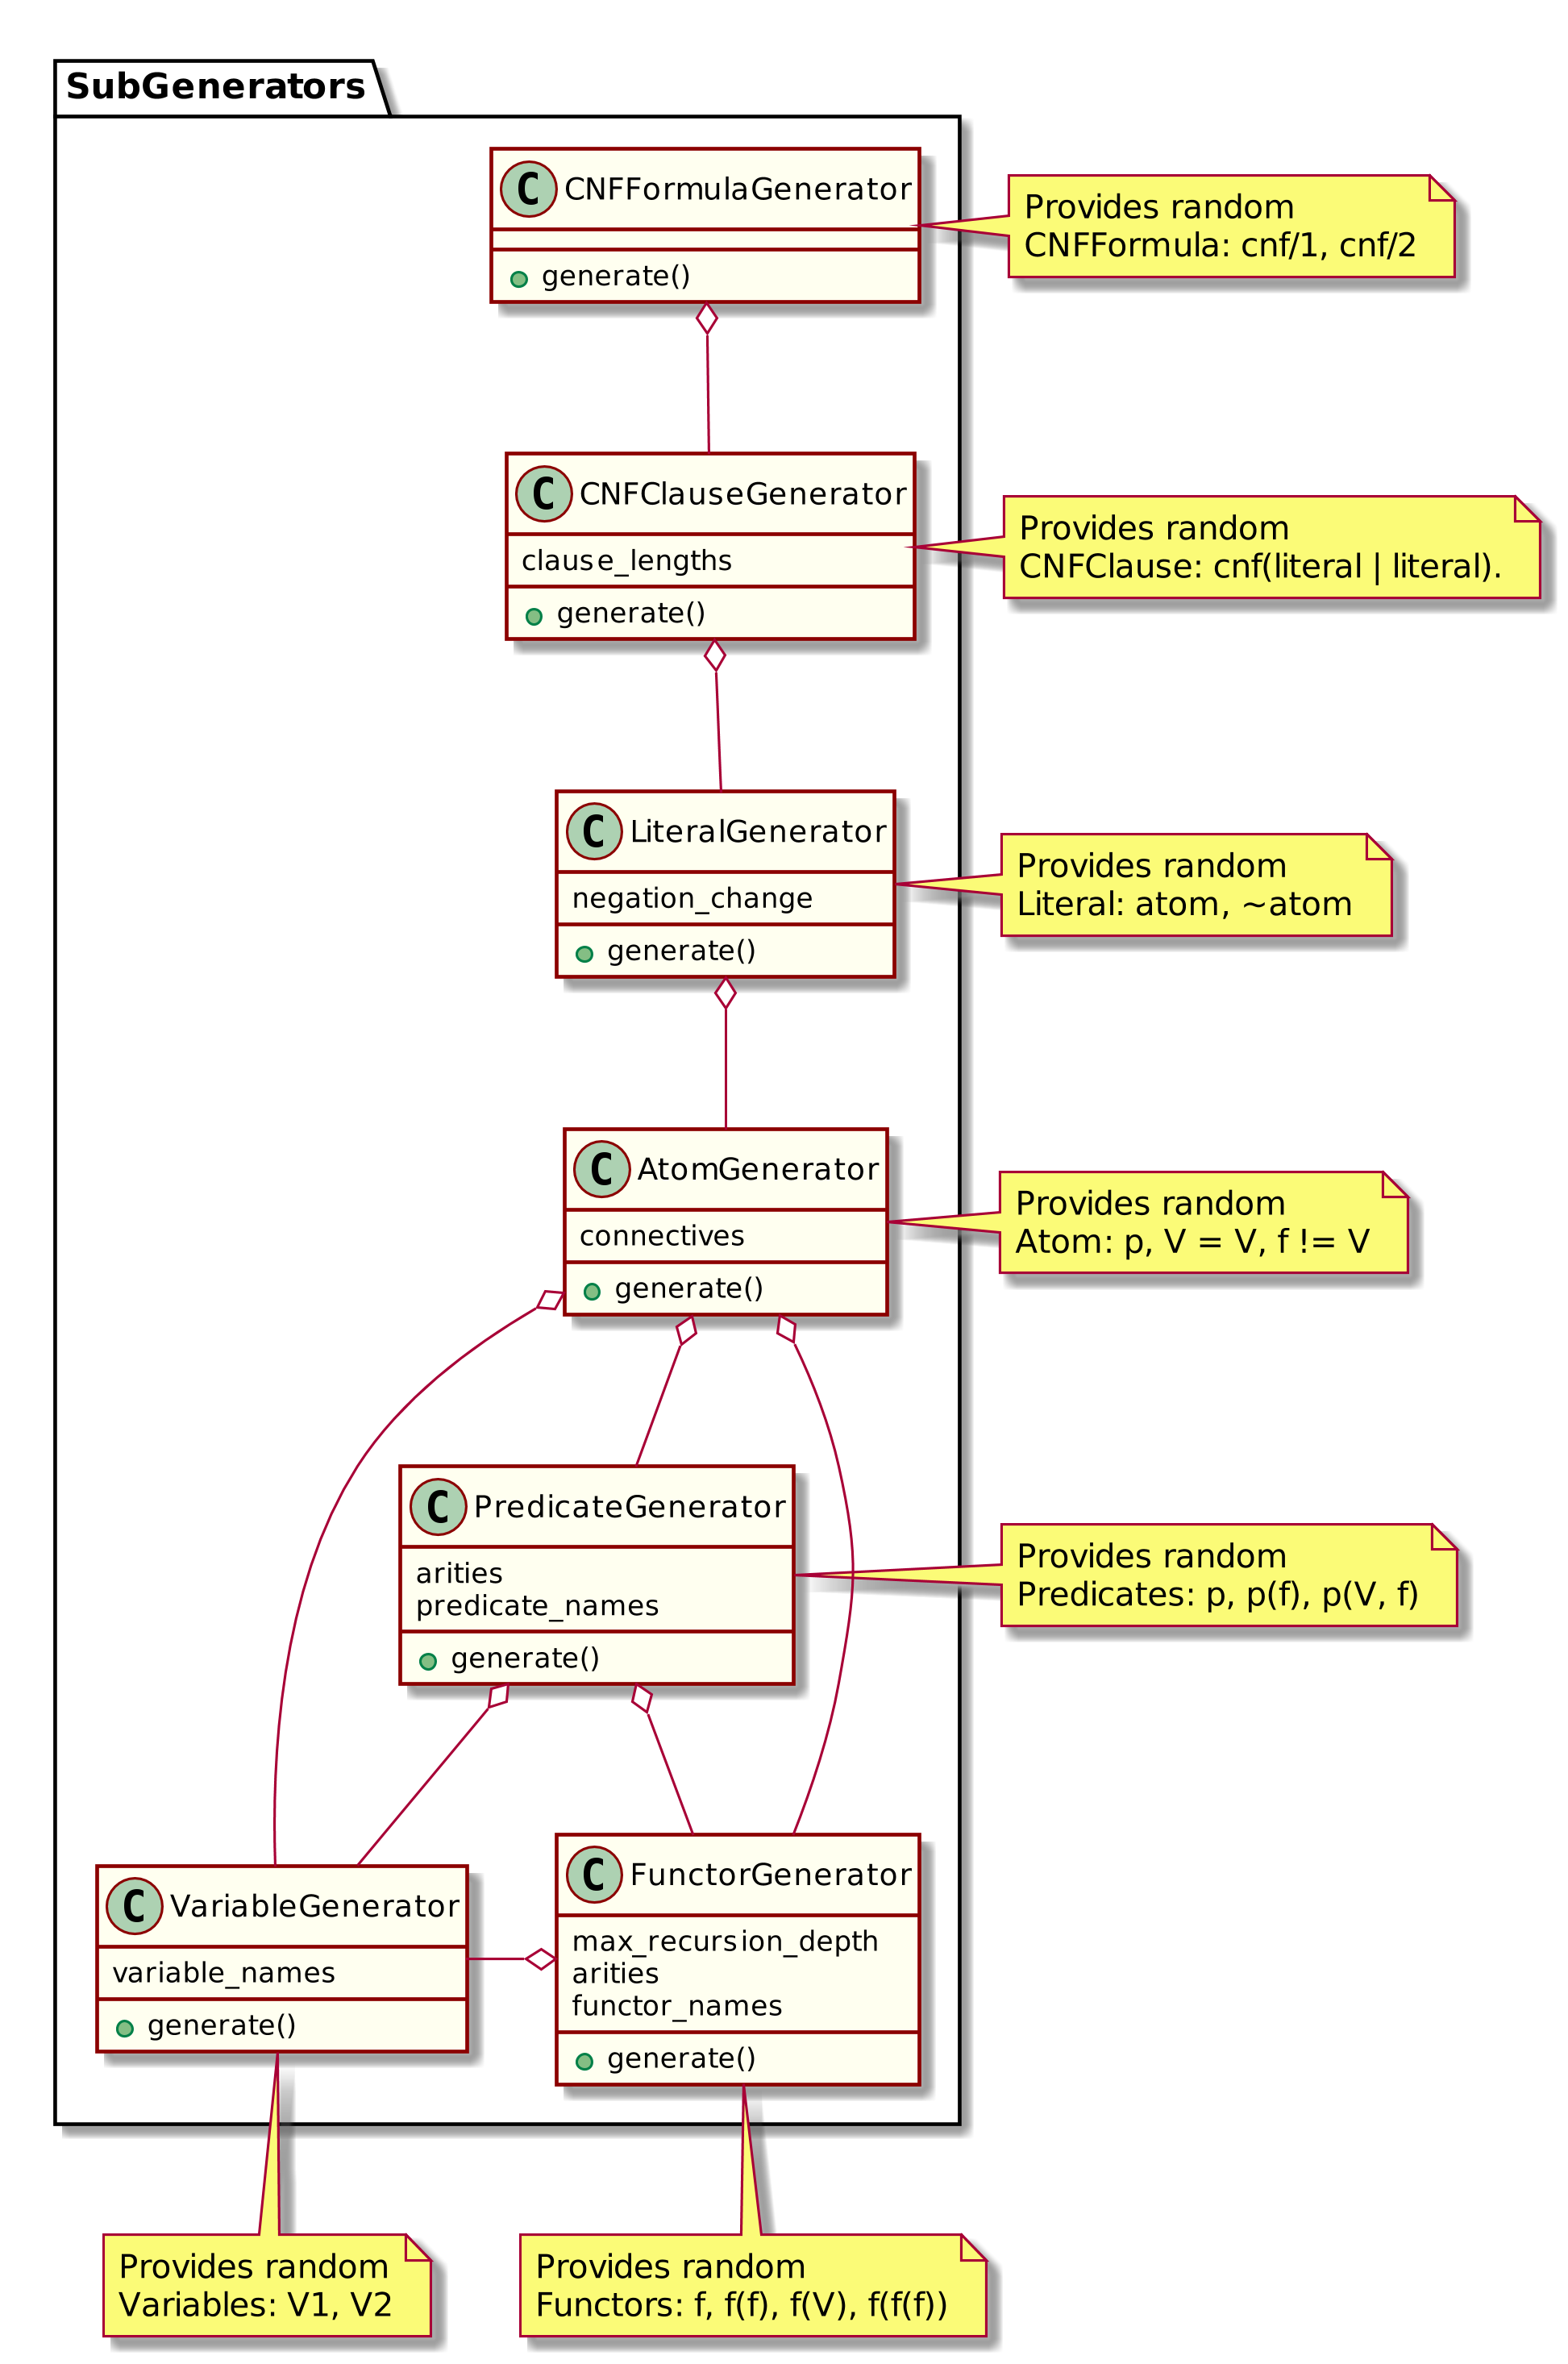
\includegraphics[width=0.8\textwidth]{logic-formula-generator/fol/cnf_signature_generators.png}
  \caption{Class diagram of SubGenerators in CNF formula generator}
  \label{pic:fol_signature_generator_class_diagram}
\end{centering}
\end{figure}

\section{Implementation of generator presets}
\label{sec:GeneratorPresets}

Subgenerators provide very fine control over generated created elements. To automate process of creating set of subgenerators a $GeneratorPreset$ can be defined. One of presets is $RandomCNFFormulaGenerator$ (picture~\ref{pic:cnf_generator_class_diagram}). This is interface for user to create random CNF formulas, it accepts all parameters defined in section \ref{sec:GeneratorParameters}.

After passing arguments to appropriate subgenerators, there are still 2 left: number of clauses and number of literals (provided as ranges). They require special care as the number of clauses affects the number of literals. To generate random formula within these constrains, number of clauses with appropriate clause length must be computed.

\begin{figure}[h]
\begin{centering}
  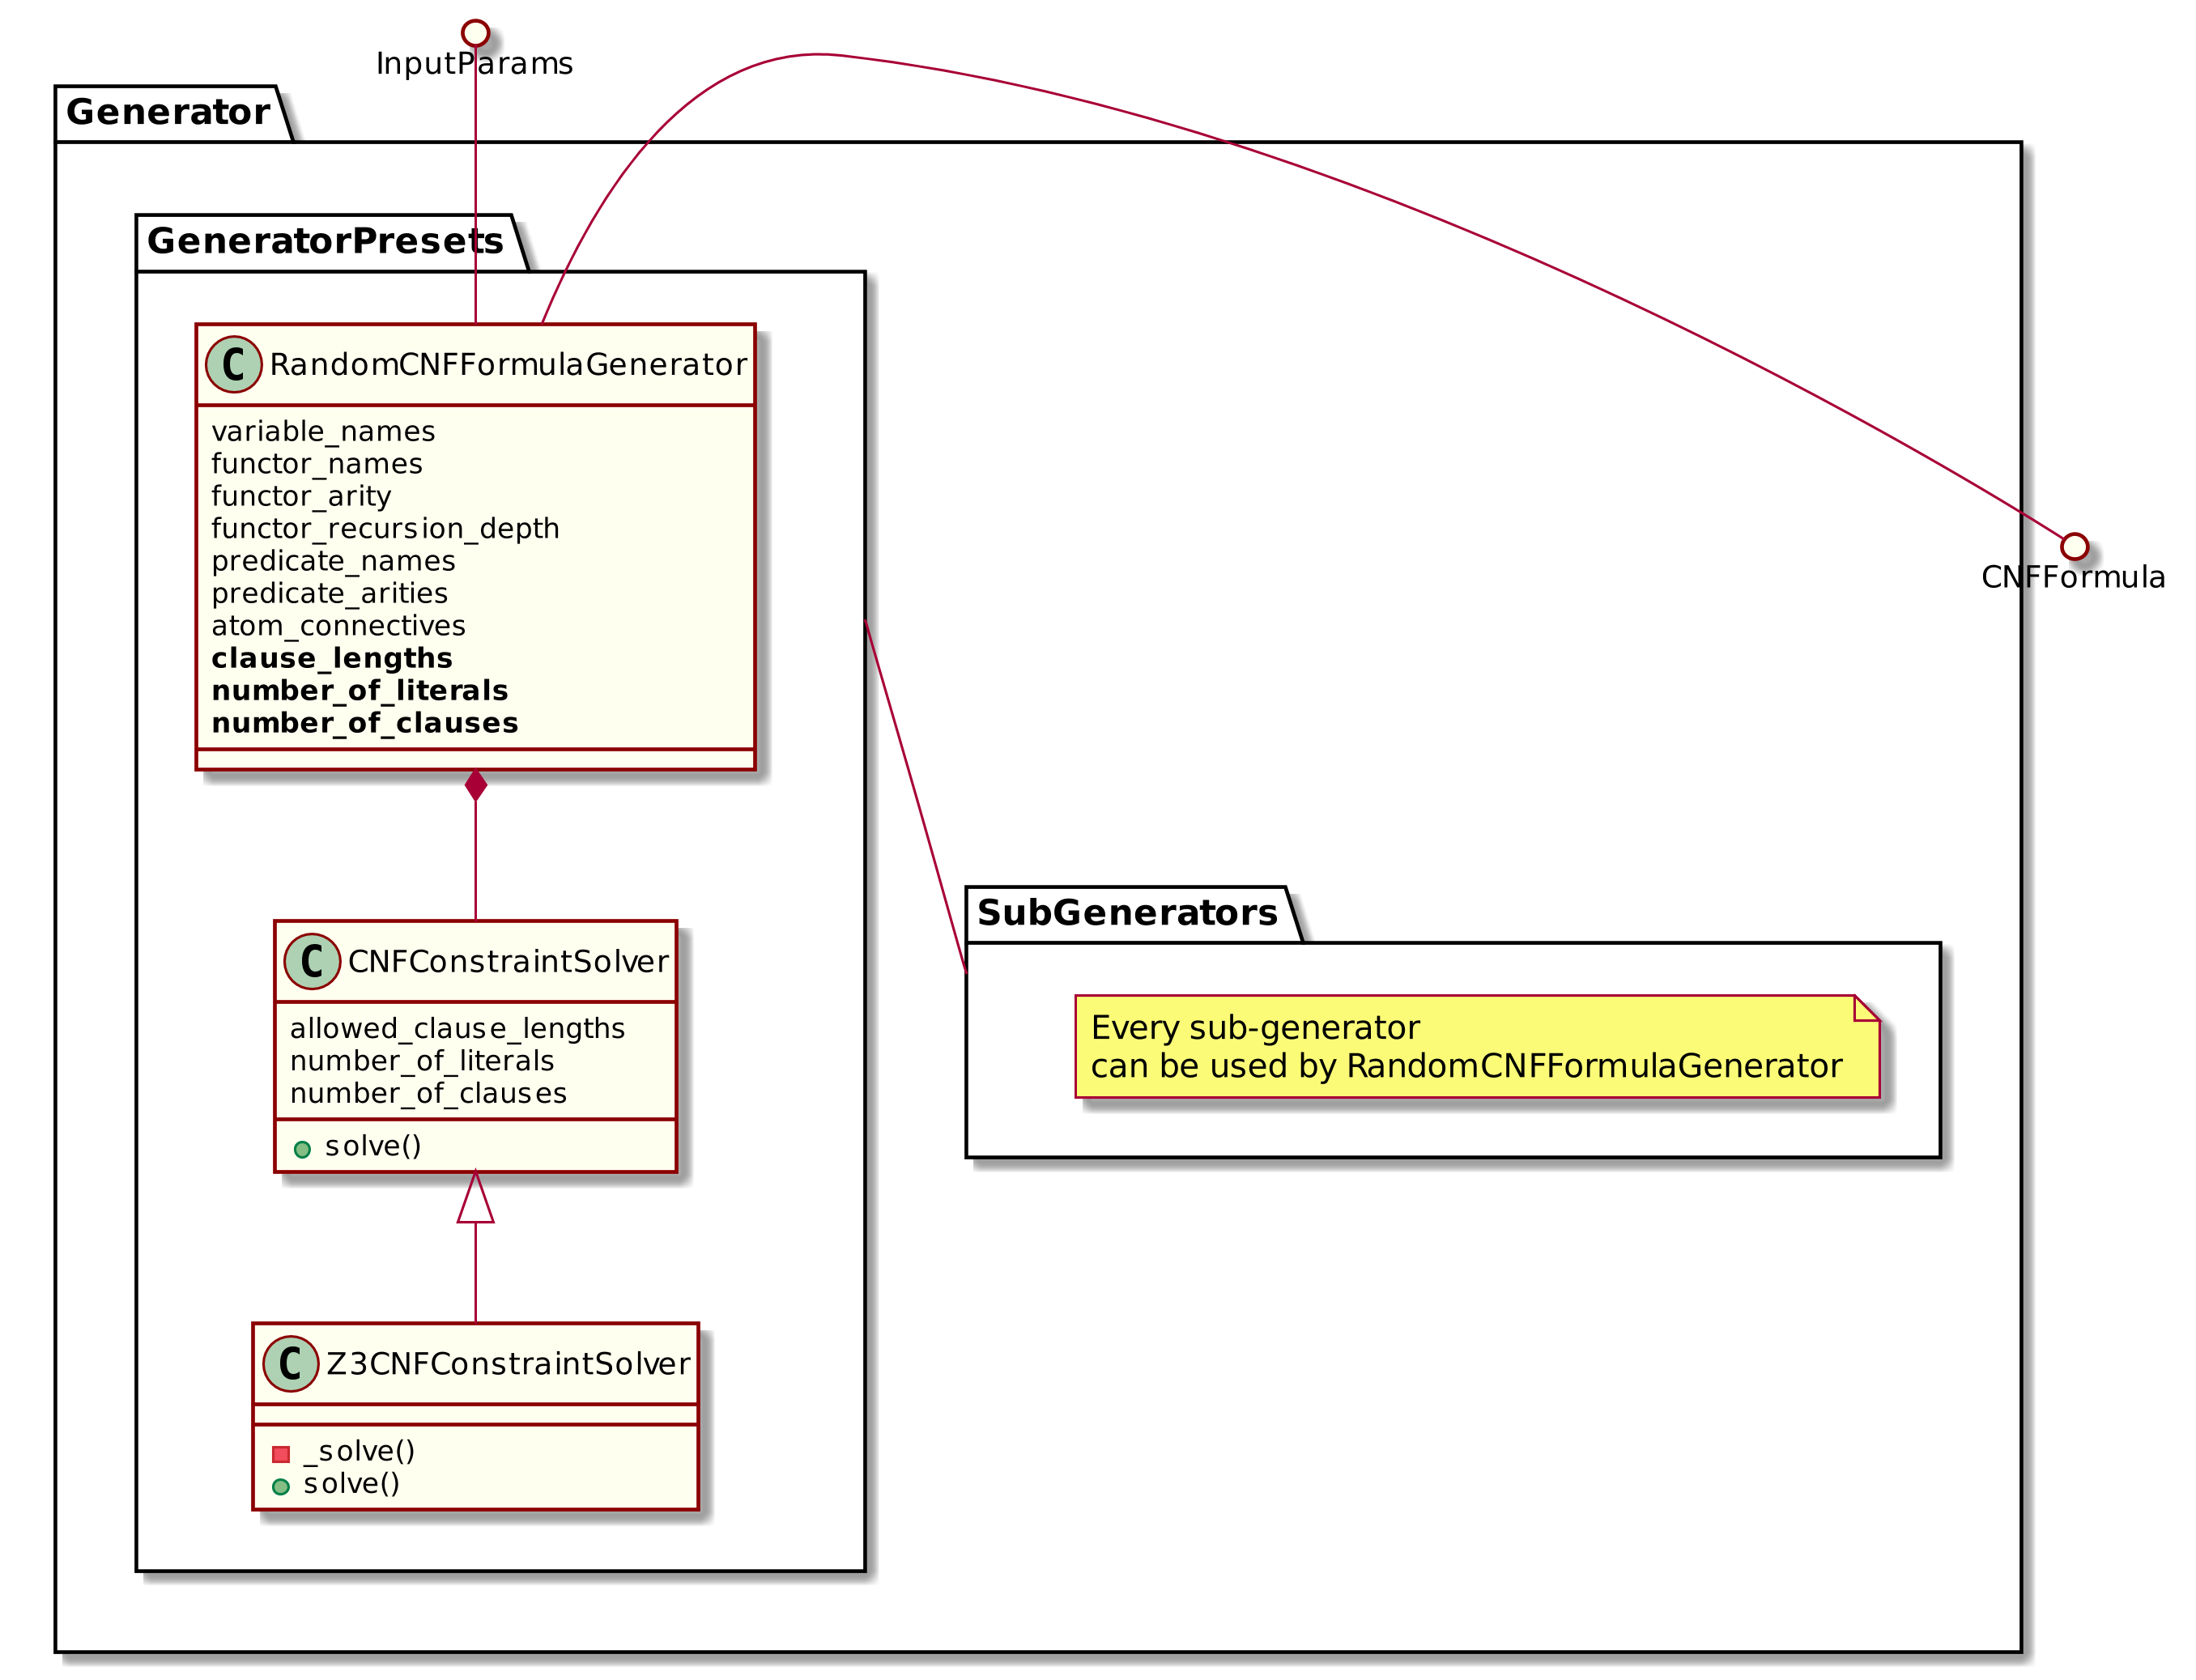
\includegraphics[width=\textwidth]{logic-formula-generator/cnf_formula_generator.png}
  \caption{Class diagram of CNF formula generator}
  \label{pic:cnf_generator_class_diagram}
\end{centering}
\end{figure}

\subsection{Randomizing formula within limits}
\label{sec:RandomizeFormulaWithinLimits}

In order to compute number of clauses with appropriate clause length, CNF formula must be formalized to create relationship between $NumberOfClauses$ and $NumberOfLiterals$.
First, define CNF formula $F_{cnf}$ as set of unordered clauses $c_1, c_2, \dots, c_n$. Computing number of clauses with this definition is trivial, but computing number of literals is not.

\begin{align*}
	&F_{cnf} = \{c_1, c_2, \dots\, c_n\}  \\
  NumberOfClauses(&F_{cnf}) = |\{c_1, c_2, \dots\, c_n\}| = n \\
	\text{where }
		&n \text{ -- number of clauses in formula}
\end{align*}

In next step, we will group clauses by their length. Let $c^m = \{c1,c2,..\}$ be set of clauses with common length $m$. Allowed clause lengths $ClauseLengths=\{1,2,..\}$ are known in advance as they were passed in input parameters. Now formula becomes sum of set of clauses grouped by length, $NumberOfClauses$ is sum of cardinality of each of clause set and $NumberOfLiterals$ can be computed similarly to $NumberOfClauses$, but number of clauses with defined length must be multiplied by its length $m$.

\begin{align*}
  &F_{cnf} = \bigcup_{m \in ClauseLengths} c^m \\
  NumberOfClauses(&F_{cnf}) = \sum_{m \in ClauseLengths} |c^m| \\
  NumberOfLiterals(&F_{cnf}) = \sum_{m \in ClauseLengths} m |c^m| 
\end{align*}

The unknown variables are $|c^m|$ - the number of clauses with length $m$. After adding constrains defined by user in input parameters:

\begin{align}
  NumberOfClauses(&F_{cnf}) = \sum_{m \in ClauseLengths} |c^m| \label{eq:UserConstraintsX}\\
  NumberOfLiterals(&F_{cnf}) = \sum_{m \in ClauseLengths} m |c^m| \label{eq:UserConstraintsLx} \\
  l_{min} < NumberOfLiterals(&F_{cnf})< l_{max} \label{eq:UserConstraintsRangeL}\\
  c_{min} < NumberOfClauses(&F_{cnf}) < c_{max}\label{eq:UserConstraintsRangeC} 
\end{align}

\subsection{Using Z3 to resolve user constraints}

Z3 \cite{Z3Solver} is a \gls{SMT} prover from Microsoft Research. It uses SMT-LIB as input format, but also has bindings to multiple languages. It can be used to solve user constraints presented in~\ref{sec:RandomizeFormulaWithinLimits}. Z3 supports integer arithmetic what is essential for solving user constraints.

Solving equation is implemented as class $CNFConstraintSolver$ (picture~\ref{pic:cnf_generator_class_diagram}). Parameter $ClauseLengths$ corresponds to equation~\ref{eq:UserConstraintsLx}, parameter $NumberOfLiterals$ corresponds to range of allowed values of literals - tuple of minimal and maximum range - (equation~\ref{eq:UserConstraintsRangeL}), parameter $NumberOfClauses$ corresponds number of allowed values of clause - tuple of minimal and maximum range - (equation~\ref{eq:UserConstraintsRangeC}). The set of variables $x_i$ will be returned from method $solve()$ as dictionary, where key is $m$ (clause length) and value is how many clauses are needed.


Function \mintinline{text}{_solve()} in listing \ref{lis:DeterministicSolve} solves user constraints using Z3 solver bindings in Python. Line 
\mintinline{python}{X = [z3.Int() ...]}
defines Z3 variables, which can contain only integer values. This variable is used to represent $x_i$ from \ref{eq:UserConstraintsX}. Further down the line 
\mintinline{python}{s = z3.Solver()} 
creates model, to which constraints will be added. Constraints are defined by functions
\mintinline{python}{z3.Sum}, 
\mintinline{python}{z3.And}, 
and can be added to model via
\mintinline{python}{s.add}.
Variables must follow 2 rules: they must be non negative and be in range defined by \ref{eq:UserConstraintsRangeC} and \ref{eq:UserConstraintsRangeL}. Solution can be calculated from model with 2 operations: first check if model is satisfayable, next evalueate (get value) of variables in model. If another solution is needed, it can be done by adding constraints, that forbids concurrencyent solution and recalculating model.


\begin{listing}[H]
  \caption{Lazy, deterministic function for solving user constraints}
  \label{lis:DeterministicSolve}
\begin{minted}{python}
    def _solve(self) -> Iterable[Dict[int, int]]:
        """Solve in deterministic order"""
        A = self.literal_coefficients
        n = len(A)
        X = [z3.Int() for i in range(n)]
        s = z3.Solver()

        # solutions must be positive
        s.add(z3.And([X[i] >= 0 for i in range(n)]))

        # clauses must be in range
        s.add(z3.Sum(X) <= self.number_of_clauses[1])
        s.add(z3.Sum(X) >= self.number_of_clauses[0])

        # literals must be in range
        s.add(z3.Sum([A[j] * X[j] for j in range(n)]) <= self.number_of_literals[1])
        s.add(z3.Sum([A[j] * X[j] for j in range(n)]) >= self.number_of_literals[0])

        while s.check() == z3.sat:
            solution = [s.model().evaluate(X[i]) for i in range(n)]
            yield {clause_len: s.as_long() for clause_len, s in zip(A, solution)}
            forbid = z3.Or([X[i] != solution[i] for i in range(n)])
            s.add(forbid)
\end{minted}
\end{listing}

Fundamental problem of using SAT (or SMT) solver in this scenario when any, random solution is needed, is fact that solver will always produce deterministic result for the same input data. There are 2 solutions for this problem. First one, presented here, is using a wrapper that will temporarily skip or discard part of solutions, to randomize deterministic output. In this cave, non public function $\_solve$ in listing~\ref{lis:DeterministicSolve} is a function that actually yields solutions and $solve$ in listing \ref{lis:RandomSolve} is a randomizing wrapper. Randomization occurs at the cost of time and memory. Second approach assumes that solver supports soft clause\footnote{contrary to hard clauses, soft clauses does not have to be satisfied}. Using soft clauses a random starting point can be suggested to a solver. For example line added to listing \ref{lis:DeterministicSolve} \mintinline{python}{s.add(z3.Sum([A[j] * X[j] for j in range(n)]) == random_number))} would hint Z3 solver to strat in \mintinline{text}{random_number} if Z3 supported this feature in Python bindings.

\begin{listing}[H]
  \caption{Lazy, randomizing wrapper around deterministic solver~\ref{lis:DeterministicSolve}}
  \label{lis:RandomSolve}
\begin{minted}{python}
    def solve(self, skip_chance: float = None):
        """Solve in random order"""
        skip_chance = random.random() if skip_chance is None else skip_chance
        cache = []
        for solution in self.solve():
            if random.random() < skip_chance:
                yield solution
            else:
                cache.append(solution)

        random.shuffle(cache)
        for cached_solution in cache:
            yield cached_solution
\end{minted}
\end{listing}


\section{Export and generate statistics about formula}
\label{sec:GenerateStatisticsAboutFormula}

After generating formula it needs to be encoded and optionally statistics can be generate. Those two things are done with visitor pattern. As input $Exporter$ receives only $CNFFormula$, as shown in picture \ref{pic:FormulaExportUtils}. First statistics are generated - $CNFFormula$ is passed to $CNFFormulaVisitor$ the result is provided as $CNFFormulaInfo$. Then $CNFFormula$ and $CNFFormulaInfo$ is handled by $TPTPExporter$ where again it is used with visitor pattern to encode formula in TPTP format. Additionally $CNFFormulaInfo$ is used to create unique to TPTP header (see for example listing \ref{lis:TPTPExample}).

\begin{listing}[h]
  \caption{Example of generated formula (limited)}
\begin{tptpcode}
% ----------------------------------------------------------------------------
% File      : 0.p 
% Syntax    : Number of clauses     :   95 ( 95 non-Horn;   0 unit;   - RR)
%             Number of atoms       :  950 (  0 equality)
%             Maximal clause size   :   10 ( 10 average)
%             Number of predicates  :   20 (206 propositional; 0-4 arity)
%             Number of functors    :   20 (940 constant;   0 arity)
%             Number of variables   :  943 (327 singleton)
%             Maximal term depth    :    0 (  - average)
% 
% ----------------------------------------------------------------------------
cnf(name,axiom,p4(V6)|p10(V1, V4, V9)|~p7|p17|p1(V4, V3, V9)|p7|p17|p1(f11, f11, f5)|p7|~p0(f2)).
cnf(name,axiom,p2(V7, V9)|p4(f19)|p2(f8, f5)|p10(f7, f8, f8)|p12|p6(V2, V6)|p14(f8, f16, f9, f16)|p3(f14, f3, f14, f18)|p11(V3, V9)|p12).
...
\end{tptpcode}
  \label{lis:TPTPExample}
\end{listing}

\begin{figure}[h]
\begin{centering}
  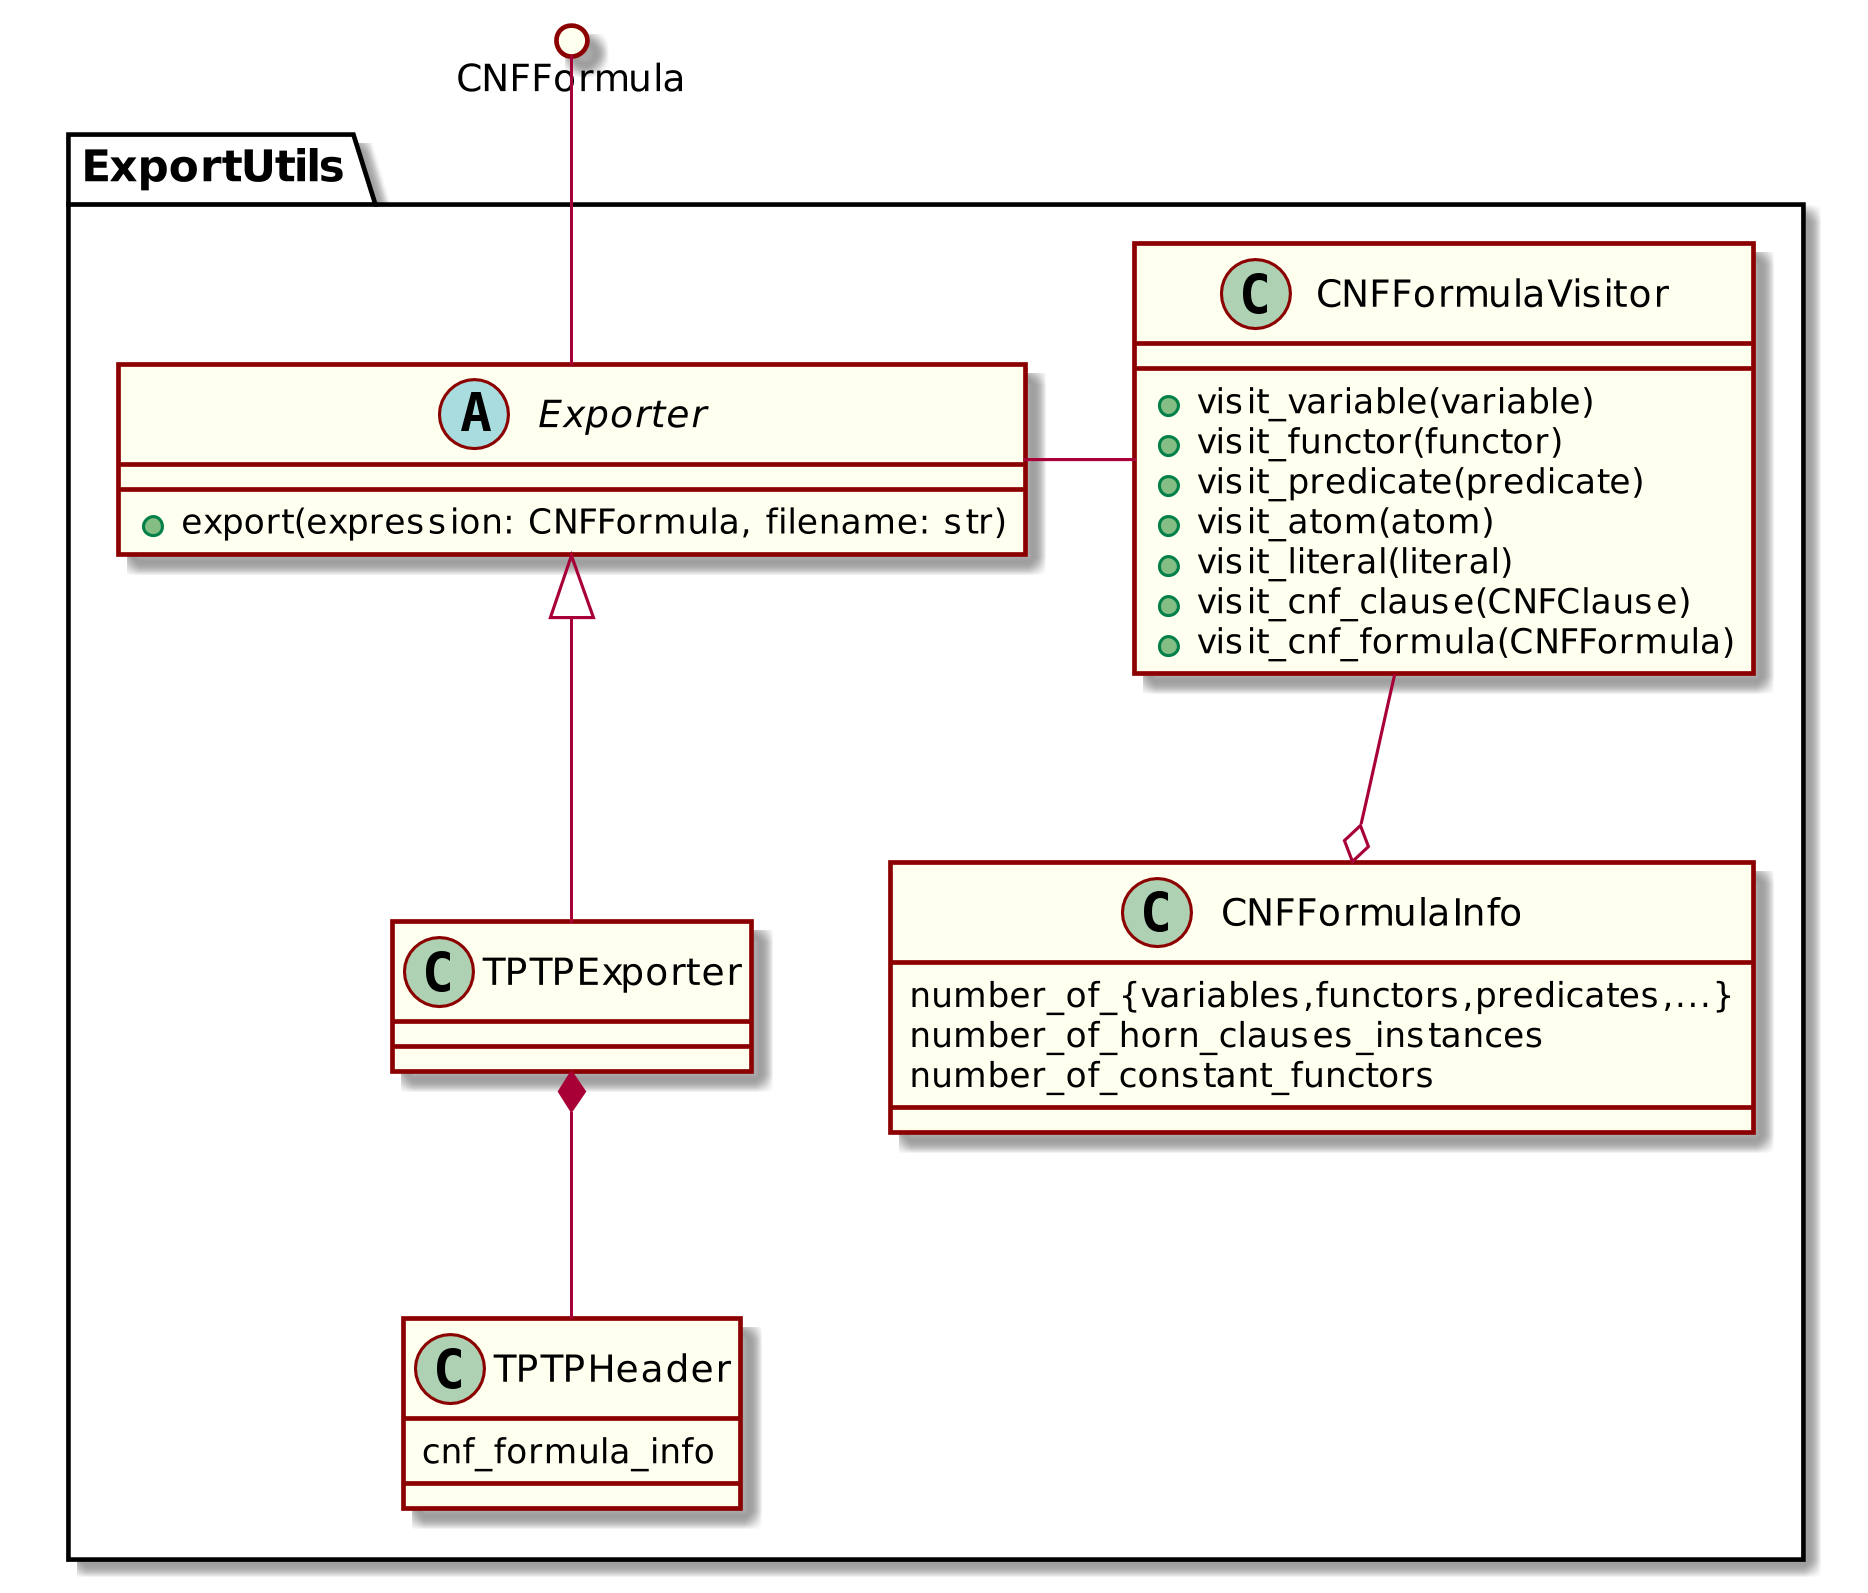
\includegraphics[width=\textwidth]{logic-formula-generator/fol/cnf_formula_statistics.png}
  \caption{Classes for which take part in generating statistics and exporting FOL CNF formula}
  \label{pic:FormulaExportUtils}
\end{centering}
\end{figure}
